\chapter{Exercise Recommendation System Based on Knowledge State}

% **************************** Define Graphics Path **************************
\ifpdf
  \graphicspath{{Chapter4/Figs/Raster/}{Chapter4/Figs/PDF/}{Chapter4/Figs/}}
\else
  \graphicspath{{Chapter4/Figs/Vector/}{Chapter4/Figs/}}
\fi

\section{Research Motivation}

%随着当今技术的飞速发展,数据量也与日俱增,人们越来越感觉在海量数据面前束手无策。正是为了解决信息过载的问题,人们提出了推荐引擎技术。推荐系统通过用户的历史行为或者用户的兴趣偏好或者用户的人口统计学特征来送给推荐算法,然后推荐系统运用推荐算法来产生用户可能感兴趣的项目列表,同时用户对于搜索引擎是被动的。目前个性化推荐技术被广泛应用于各个行业,它大大节省了用户获取信息的成本,也方便了信息提供商对用户的定向信息推送,因此大大加速了社会的信息交流效率,从而推动了传媒、娱乐、教育等基于信息交流的行业的发展。在教育领域,推荐系统的应用仍停留在较为初级的阶段,很多情况下还依赖人工筛选教育资源进行推荐,这种推荐方式效率低、成效差,且出于成本的原因也无法覆盖到所有的学生。随着推荐系统技术的成功应用和教育行业的进一步成熟,将以往通过人工实现的教育资源推荐系统改用智能化技术来进行的阻力越来越小。在国家提倡智慧教育、精准教学、智慧学习的背景下,一款成熟的具备实用价值的自适应习题推荐系统成为教育业者的期待。

%本章的目的是基于前两个章节所挖掘出的习题知识点和知识状态进行习题推荐,其核心是基于学生的知识状态,寻找出对学生当前知识掌握度改善最大的习题进行推荐,即习题推荐以查漏补缺为目的。因此获取学生的知识状态和习题涉及的知识点是本章前提。但是目前的习题库往往过于庞大,因此,从海量的习题推荐资源中直接应用推荐算法会出现效率较低的情况,不利于商业化大规模部署。在匹配阶段,根据用户特征,从海量的习题库中,快速筛选出一部分潜在适合的习题作为粗筛集合。在排序阶段,将提出的推荐模型应用于粗筛习题集,输出一个按照优先级排序的推荐习题集列表。


With the rapid development of today's technology, the amount of data is increasing day by day, and people increasingly feel helpless in the face of massive amounts of data. It is precisely in order to solve the problem of information overload that people propose the recommendation engine technology. The recommendation system sends the recommendation algorithm to the recommendation algorithm through the user's historical behavior or the user's interest preferences or the user's demographic characteristics, and then the recommendation system uses the recommendation algorithm to generate a list of items that the user may be interested in. At the same time, the user is passive to the search engine. At present, personalized recommendation technology is widely used in various industries. It greatly saves the cost for users to obtain information, and it also facilitates information providers to push targeted information to users. Therefore, it greatly accelerates the efficiency of social information exchange, thereby promoting media, The development of industries based on information exchange, such as entertainment and education. In the education field, the application of the recommendation system is still at a relatively primitive stage. In many cases, it still relies on manual screening of educational resources for recommendation. This recommendation method is inefficient, poorly effective, and cannot cover all of them due to cost reasons. student. With the successful application of the recommendation system technology and the further maturity of the education industry, the resistance to the use of intelligent technology in the education resource recommendation system implemented manually in the past is becoming less and less. In the context of the country's promotion of smart education, precise teaching, and smart learning, a mature and practical self-adaptive exercise recommendation system has become the expectation of the education industry. For the purpose of improving education and teaching, this chapter proposes an exercise recommendation model based on students' knowledge mastery.

The purpose of this chapter is to recommend exercises based on the knowledge points and knowledge status of the exercises excavated in the first two chapters. The core is to find the exercises that improve the students' current knowledge mastery the most for recommendation based on the student's knowledge status, that is, exercises It is recommended to check for omissions and fill vacancies. Therefore, acquiring the knowledge status of students and the knowledge points involved in the exercises is the premise of this chapter. However, the current exercise database is often too large. Therefore, directly applying the recommendation algorithm from the massive exercise recommendation resources will have low efficiency and is not conducive to commercial large-scale deployment. Therefore, this paper proposes a recommendation model based on two stages of matching and ranking. n the matching stage, according to the user's characteristics, a part of the potentially suitable exercises is quickly screened out from the massive exercise library as a coarse sieve set, and then based on the coarse sieve set, the proposed recommendation algorithm model is applied to recommend exercises. In the matching stage, according to the characteristics of users, a part of the potential suitable exercises can be quickly screened out as a coarse screening set from the massive exercise library. In the ranking stage, the proposed recommendation model is applied to the coarse screening exercise set, and a list of recommended exercise sets sorted by priority is output.

\section{Proposed Model}
\subsection{Algorithm Overview}
%本章提出一个基于Matching-Ranking-Feedback三个阶段的数学习题推荐模型,它针对习题库过于庞大导致推荐效率低下的问题,提出了一种基于协同过滤的习题匹配筛选算法用于筛选出一个小规模的习题候选集合。

This chapter proposes a recommendation model based on three stages of Matching-Ranking-Feedback. It addresses the problem of low recommendation efficiency caused by too large exercise database, and proposes a collaborative filtering-based exercise matching screening algorithm to filter out a small scale The candidate set of exercises.

% 分为以下几个部分:第一部分为召回部分,即候选试题生成,它产生一系列相似的习题,这是通过图神经网络来对试题进行聚类来进行,它应用图聚类方法,将试题基于知识点来进行合理聚类。第二部分为排序部分,它结合知识追踪系统获取的学生的知识状态,并结合协同过滤算法,来生成一个Top N的习题推荐列表;第三部分为反馈部分,学生做的推荐的习题又回继续输入到知识追踪系统和推荐系统中。
%1. 练习候选生成。这部分的作用是生成一系列符合学生当前学习状态的练习,并快速筛选出一组初步的练习,后续部分将从这组练习中生成最合适的N个练习,并通过协同过滤算法进行排序。它参考youtube推荐系统设计了一个多层MLP网络。它将知识跟踪生成的学生学习状态嵌入向量与学生的问题记录嵌入、个性化信息等并联作为输入。经过一系列的ReLU网络,然后通过softmax归一化输出所有候选练习的概率分布。
%2. 第二部分该部分用与上一部分类似的神经网络架构,实现了对推荐试题的排序。它的输入是用户的知识结构,最近练习,以及相似用户的常见练习题。

This chapter proposes an adaptive test question recommendation method combining graph neural network knowledge tracking and collaborative filtering. This method uses the GAT knowledge tracking model designed in the previous chapter to model the student’s knowledge state, and uses the graph neural network clustering method to cluster the test questions based on knowledge points, so as to obtain a series of related exercise. The first part is the matching part, i.e., candidate test generation, which generates a series of similar exercises, and this is done by clustering the test questions through graph neural networks, which apply graph clustering methods to cluster the test questions based on knowledge points in a reasonable way. The second part is the ranking part, which combines the knowledge state of students obtained from the knowledge tracking system with co-filtering.
\begin{enumerate}
  \item Exercise candidate generation: The role of this part is to generate a series of exercises that match the student's current learning state, and quickly filter out a preliminary set of exercises, and the subsequent part will generate the most suitable N exercises from this set and sort them by collaborative filtering algorithms. It designs a multi-layer MLP network with reference to the youtube recommendation system. It concatenates the student learning state embedding vector generated by knowledge tracking with the student's problem record embedding, personalized information, etc.\ as input. After a series of ReLU networks and then output a probability distribution over all candidate exercises by softmax normalization.
  \item Ranking: This part is to generate Top N recommendation exercise. It implements the ranking of the recommended test questions using a neural network architecture similar to that of the previous section. Its inputs are the user's knowledge structure, recent exercises, and common practice questions from similar users.
\end{enumerate}

The structure of the recommendation system is like \figurename{\ref{fig:ch4-fig0}}

\begin{figure}[h]
  \centering
  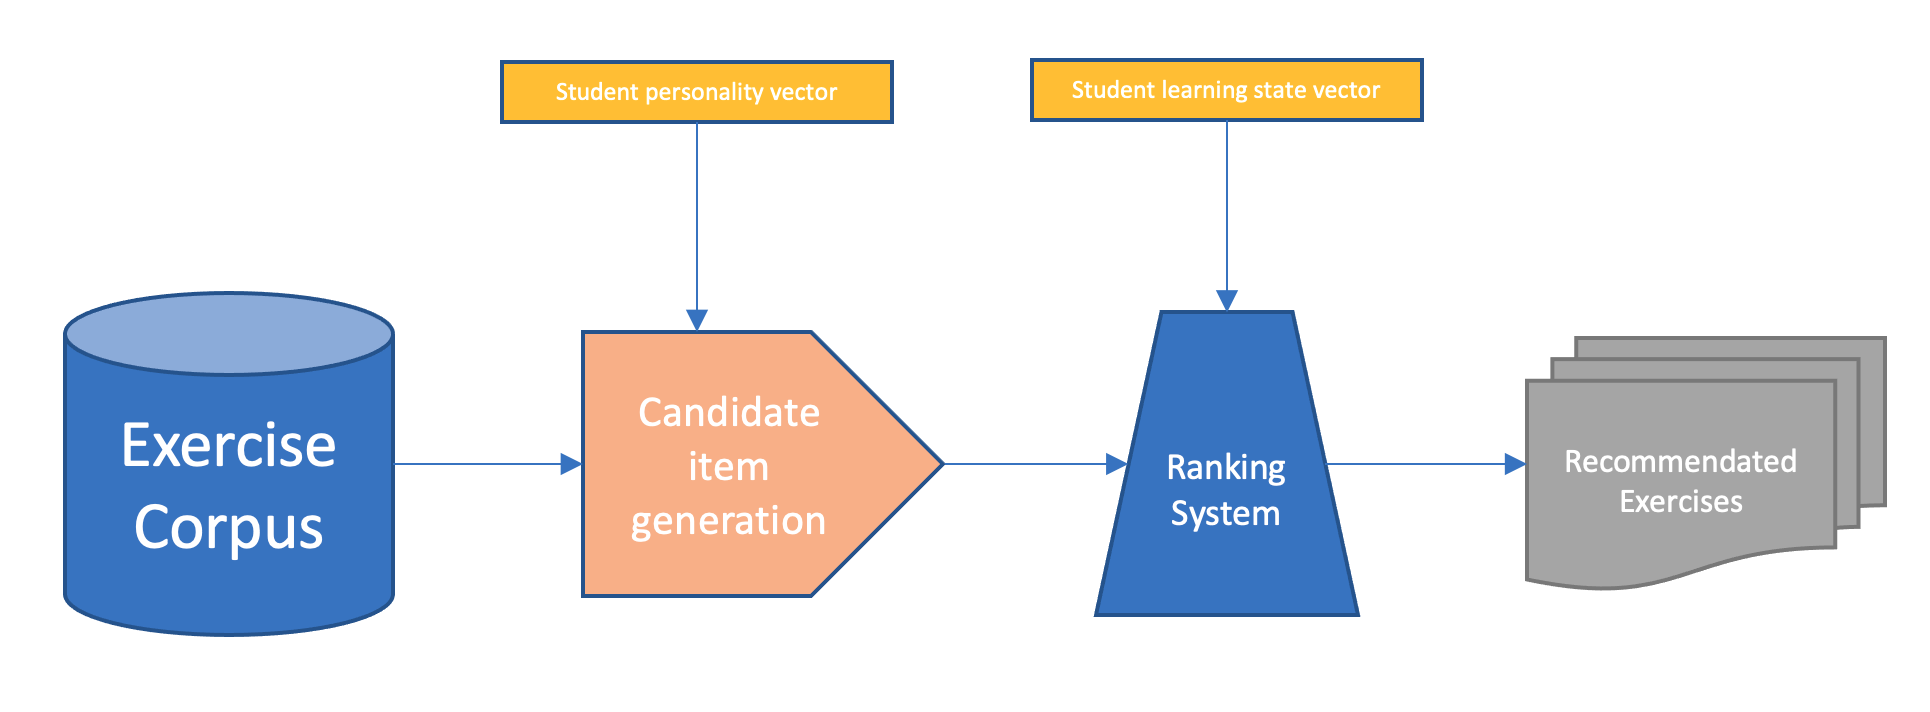
\includegraphics[width=1.0\textwidth]{ch4-fig1.png}
  \caption{The Architecture of Recommendation System}\label{fig:ch4-fig0}
\end{figure}

\subsection{matching Stage}
In the matching phase, due to the large amount of data, the algorithm of Collaborative Filtering (CF)\cite{salakhutdinov2007restricted} can achieve half the result with twice the effort. It only needs to calculate the similarity of students' knowledge states \(h^\prime \) with other students who have similar knowledge states \(h\).

Collaborative Filtering, the most classic type of recommendation algorithm, includes both online collaborative and offline filtering. The so-called online collaborative is to find items that users may like through online data, while offline filtering is to filter out data that are not worth recommending, such as data with low recommendation value ratings, or data that users have already purchased despite high recommendation values. The model of collaborative filtering is generally m recommended items, m users' data, only some users and some data are rated between the data, other parts of the rating is blank, at this time we want to use the existing part of the sparse data to predict the rating relationship between those blank items and data to find the highest rated items recommended to users.

Generally speaking, there are three types of collaborative filtering recommendations. The first one is user-based collaborative filtering, the second one is item-based collaborative filtering, and the third one is model-based collaborative filtering.


\subsubsection{Student Similarity Calculation}
The purpose of collaborative filtering is to recommend recommended items of users similar to the target user to the user. The user-based collaborative filtering algorithm is discovered through historical behavior data of users, and measures and scores these preferences. Set the similarity of users through a given algorithm, and make recommendations among users who have the same preferences.

User-based collaborative filtering mainly considers the similarity between users and users. As long as we find out the items that similar users like and predict the target users' ratings of the corresponding items, we can find the items with the highest ratings and recommend them to users. The item-based collaborative filtering is similar to the user-based collaborative filtering, except that we turn to find the similarity between items and users, and only if we find the ratings of certain items by target users, then we can predict similar items with high similarity and recommend the highest rated similar items to users. For example, if you buy a machine learning related book online, the website will immediately recommend a bunch of machine learning, big data related books to you, and the idea of collaborative filtering based on items is obviously used here.

Similar statistics are used to get neighboring users with similar hobbies or interests, so we can use the obtained user's knowledge state embedding \(h_t\) from the previous knowledge tracking module, which can be used as the basis for calculating the similarity. The first step is to find other users who are similar to the new user based on their historical behavior information; at the same time, to predict the items that the current new user may like based on the evaluation information of these similar users on other items. Given the user rating data matrix R, the user-based collaborative filtering algorithm needs to define the similarity function \(s : U \times U \to R\) to calculate the similarity between users, and then calculate the recommendation results based on the rating data and the similarity matrix. We can use the cosine similarity to calculate this value.

\begin{align}
  s(u, v)=\frac{h_{u} \cdot h_{v}}{\|h_{u}\|_{2}\|h_{v}\|_{2}}
\end{align}
where \(h_u\) and \(h_v\) represent the knowledge mastery state of user \(u\) and \(v\).
We can obtain the exercise recommendation history \(\mathcal{H}\) of user B, which is closest to user A to be recommended, and then use the exercises in \(\mathcal{H}\) as a rough set as the next sorted list of exercises.

\subsubsection{Exercise Filtering System}
Through the previous section, we calculated the similarity of students, which comprehensively considers students' current knowledge proficiency, students' personalized information and so on. Next, we need to use the collaborative filtering algorithm to generate a rough recommended set of exercises \(S_{raw}\).

When the recommendation system is running, the system will record the students' question records. After calculating the similarity of the students, they can be sorted according to the similarity. Given a threshold, list the students whose similarity is greater than the threshold, and divide the students according to the list. The exercises corresponding to the problem record are added to \(S_{raw}\).

The algorithm is as~\ref{alg:EF}:
\begin{algorithm}[h]
  \caption{Exercise Filtering Algorithm}\label{alg:EF}
  \begin{algorithmic}
    \REQUIRE~~\\
    The target student \(s_i\); \\
    The student represent matrix, \(S=\{s_0,s_1,\ldots,s_N\} \);\\
    The log of recommendation \(L=\{L_0,L_1,\ldots,L_N\} \) \\
    The log-exercise relation: \(L_i=\{E_0,\ldots,E_{|L_i|}\} \) \\
    The filtering thread \(T\);
    \ENSURE~~\\ %算法的输出:Output
    The filtered exercise set \(S=\{E_{s_0},\ldots,E_{s_N}\} \)
    \STATE~Calculate the similarity between \(s_i\) and other students \(Sim\)
    \STATE~Sort \(Sim\) and get the top \(T\) results \(R=\{s_{r_0},\ldots,s_{r_T}\} \);
    \STATE~Aggregate the exercises log of students in \(R\), get exercise set \(S\)
    \RETURN~\(S\); %算法的返回值
  \end{algorithmic}
\end{algorithm}




\subsection{Ranking Stage}
%本节我们设计了一个基于MLP的试题排序模型,该模型输入学生的知识状态向量$h_t$,以及通过序列嵌入学习的知识状态改变向量$d_h$,以及习题的知识点标注向量。

In the previous step we obtained a list of recommended exercises for similar students by collaborative filtering in the matching phase, and in this phase, a ranking of the exercises is needed to further reduce the amount of recommendations and give the ranking sequence of exercise. In this section, we design an MLP-based test ordering model. The model inputs the student's knowledge state vector \(h_t\), the knowledge state change vector \(d_h\) learned through sequence embedding, and the knowledge point labeling vector of the exercises. The architecture is like \figurename{\ref{fig:ch4-fig3}}.


\begin{figure}[h]
  \centering
  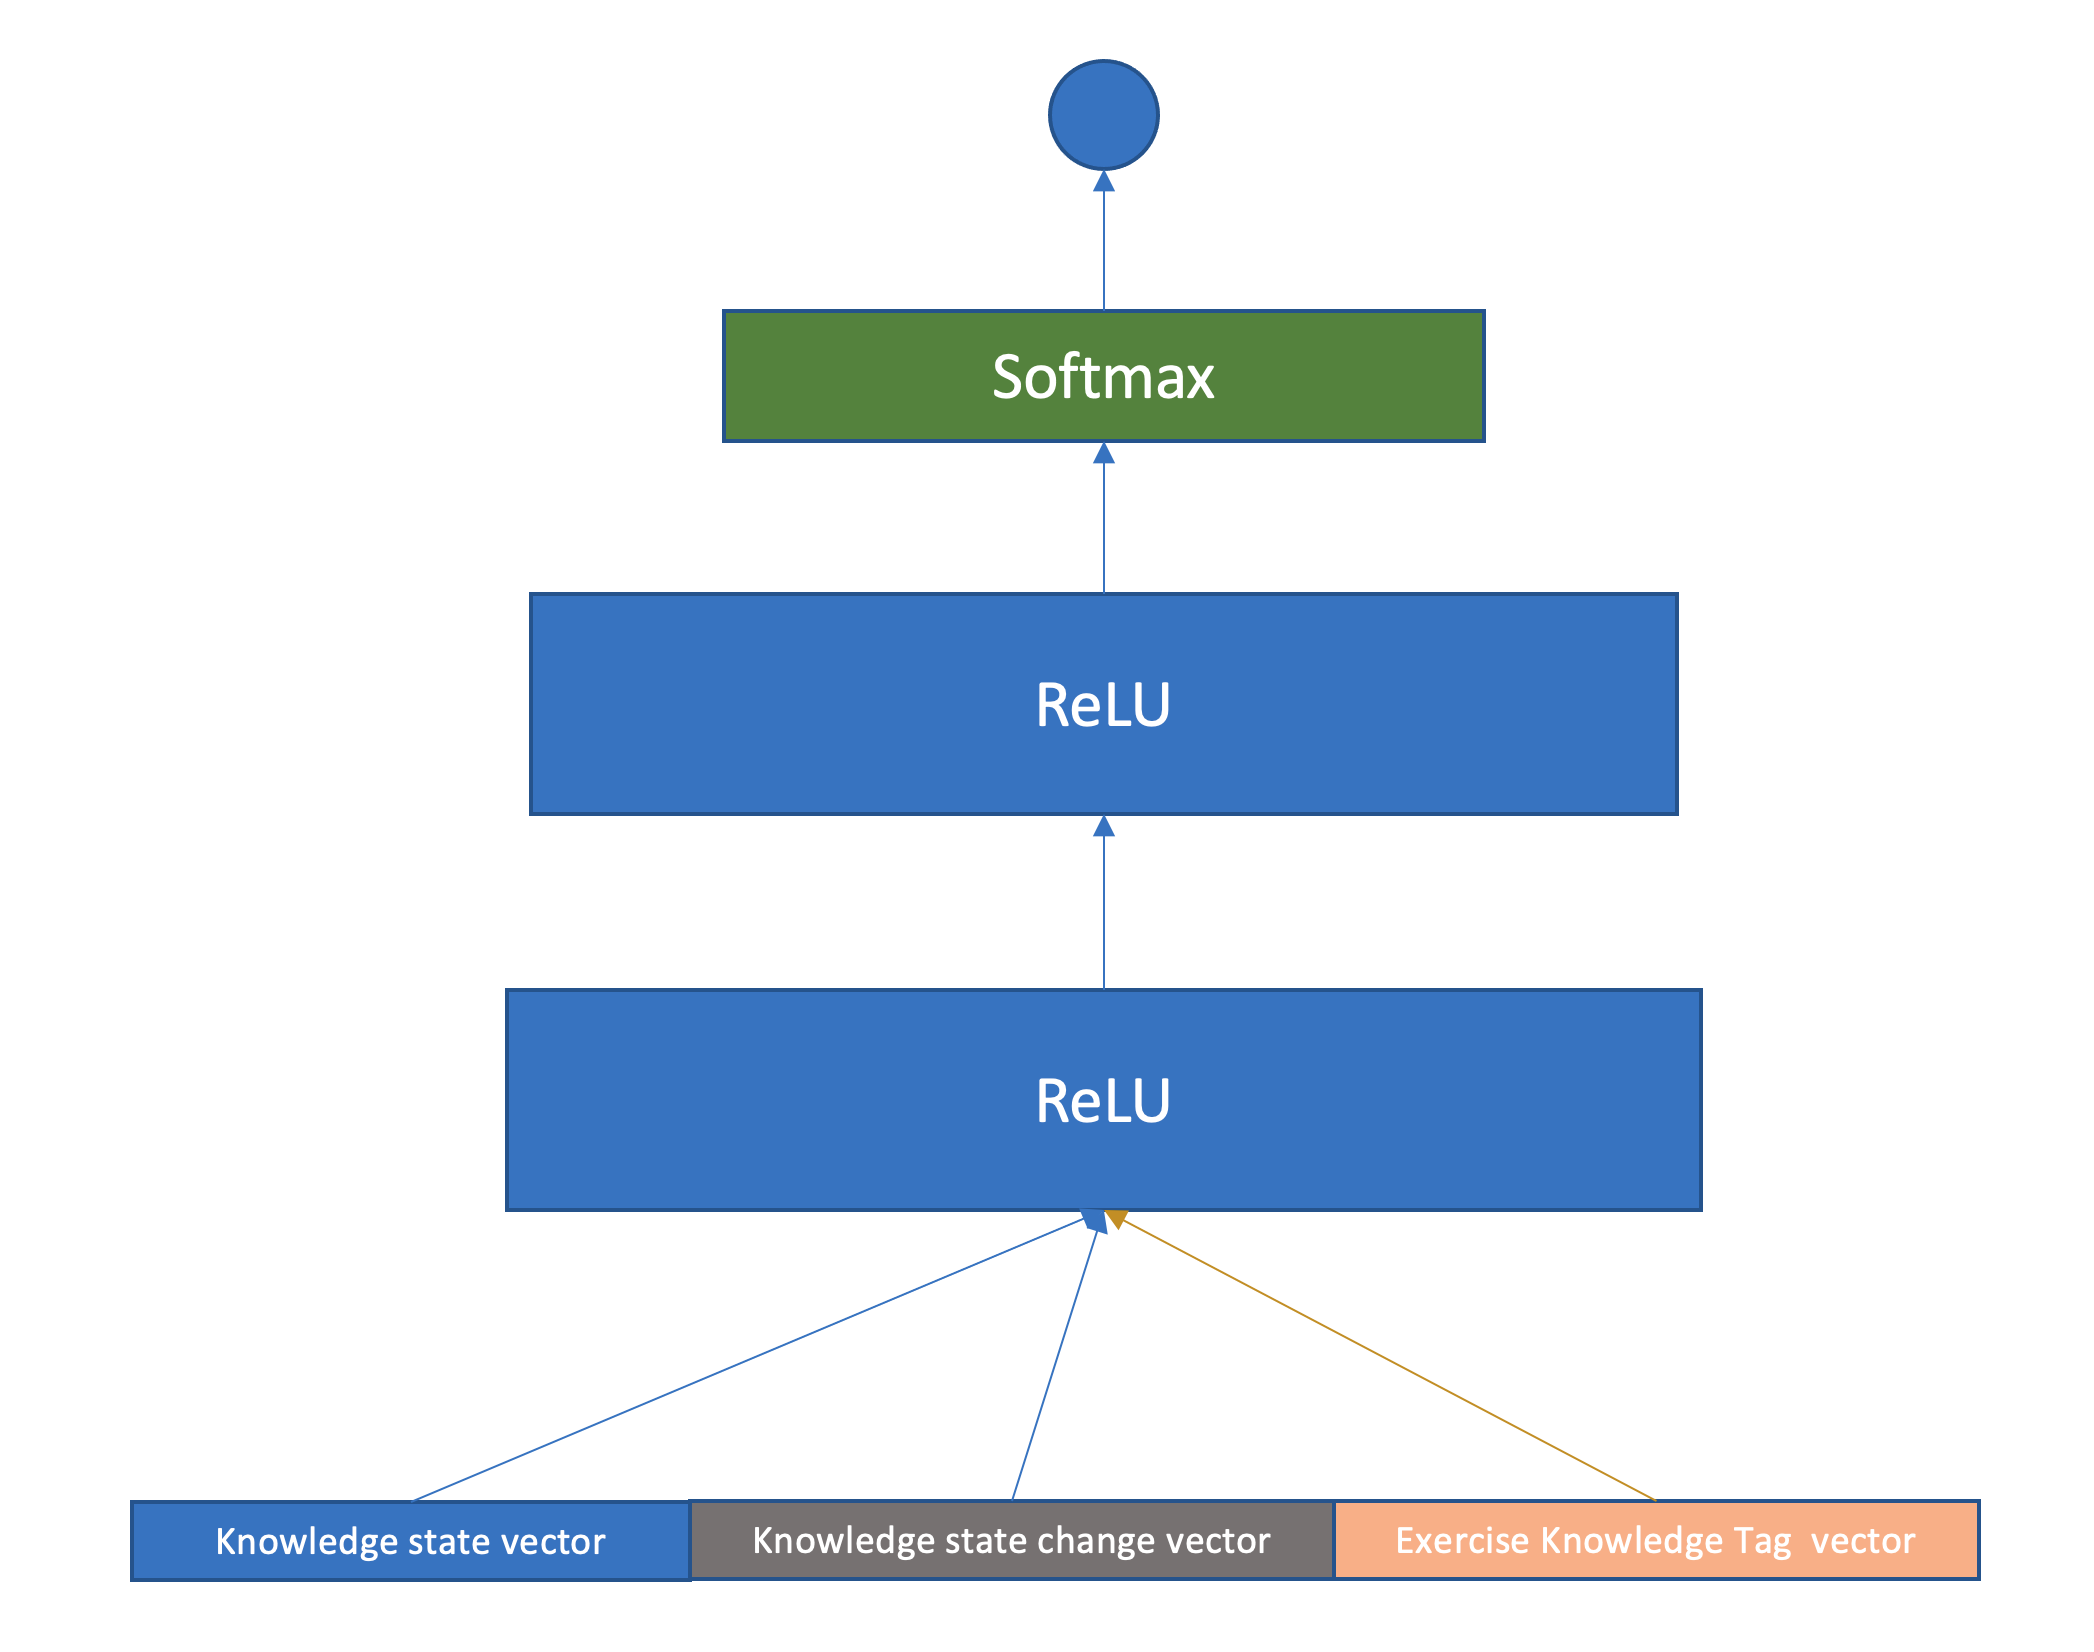
\includegraphics[width=1.0\textwidth]{ch4-fig3.png}
  \caption{The Architecture of Recommendation System}\label{fig:ch4-fig3}
\end{figure}

The model is a three-layer multi-layer perceptron, with two fully connected layers in the middle, and the output layer uses softmax to output the probabilities of exercise recommendation. The input layer inputs the student's knowledge state vector, knowledge state change vector and exercise knowledge point label vector. The model is a three-layer multi-layer perceptron, with two fully connected layers in the middle, and the output layer uses softmax to output the probabilities of exercise recommendation. The input layer inputs the student's knowledge state vector, knowledge state change vector and exercise knowledge point label vector. The loss function is:
\begin{align}
  \mathcal{L}=\sum_{i=1}^{T} y_i \log (\text{sigmoid}(\hat{y}_i))+(1-y_i ) \log (1-\text{sigmoid}(\hat{y}_i))
\end{align}
where \(\hat{y}_i\) is the output value, \(y_i\) is actual recommended weights for the exercises.

After training the model, sort the output values, and the sorted list is the recommended problem set.
%在训练好模型之后,将输出值进行排序,排序的列表即为推荐的习题集。


\section{Experiment}
%本模型的核心思想是为学生查漏补缺,因此,在学生的知识状态一定的情况下,尽量给学生推荐对其知识掌握情况带来正向收益最大的习题。
\subsection{Dataset}
%考虑到本推荐系统需要立足于学生的知识状态针对习题进行推荐。目前市面上并没有

\section{Summary}
%本节提出了一个基于召回-排序的双阶段推荐系统框架,在召回阶段,采用了协同过滤的方式,排序阶段,则采用了多层感知机,来对学生知识状态-习题知识点进行建模,同时考虑到学生的学习速度即知识状态改变,输出习题与当前知识状态匹配度。
This section proposes a two-stage recommendation system framework based on matching-ranking. In the matching stage, collaborative filtering is used, and in the ranking stage, multi-layer perceptron are used to model students' knowledge state-exercise knowledge points. At the same time, taking into account the student's learning speed, that is, the change of knowledge state, the output exercises match the current knowledge state.